\documentclass[10pt,a4paper]{article}
\usepackage[latin1]{inputenc}
\usepackage{amsmath}
\usepackage{amsfonts}
\usepackage{amssymb}
\usepackage{graphicx}
\usepackage{listings}
\usepackage{color}

\lstset{frame=tb
	language=Fortran
	  aboveskip=3mm,
	  belowskip=3mm,
	  showstringspaces=false,
	  columns=flexible,
	  basicstyle={\small\ttfamily},
	  numbers=none,
	  numberstyle=\tiny\color{gray},
	  keywordstyle=\color{blue},
	  commentstyle=\color{dkgreen},
	  stringstyle=\color{mauve},
	  breaklines=true,
	  breakatwhitespace=true,
	  tabsize=3
}


\title{Molecular Dynamics - a Simulation of Argon Gas}
\date{March 18, 2015}
\author{Scott O'Connor}

\begin{document}
\maketitle

\begin{abstract}
	An argon gas Lennard Jones Potential simulation is presented. Verlet Velocity Integration is utilized to determine the position and velocity of each particle. The gradient of the Lenard Jones potential is used to calculate the pair-wise forces of the particles. 
\end{abstract}

\section{Intro}
Molecular dynamics simulations calculate the pairwise interactions of particles due to various potentials. The Lennard Jones potential, describes the interaction of two neutral atoms. LJ has two terms which comes from Pauli Repulsion and dipole-dipole iterations. This model is often used due to its simplicity.

The gradient of the potential results in the force between the two particles. Since the mass of all particles are known, the acceleration of each particle can be calculated. The acceleration, is then integrated to find the velocity and position of the particle.

Several types of integrators can be used in the md simulations. Each integrator has certain properties that make it favorable.The varlet velocity integrator was chosen because of its ability to conserve energy. 

Initial positions and velocities are critical for a successful simulation. The initial position of the gas molecules is in a fcc cell. The distance between each of the molecules should be in the lowest state possible and therefore at a distance of sigma. Sigma sits at the bottom of the potential well or at $2^{1/6}$ if all constants are normalized to 1.

The initial velocity of the gas molecules will be a normal distribution such that the center of mass of the system is preserved. Fortran STL comes with only a uniform random number generator. To change the uniform random numbers outputted from the generate to normal random numbers a box muller transform needs to be utilized. To correct for an changes in the center of mass, the sum of the momentum is normalized by the number of particles and subtracted. This results in zero net momentum in any direction.


\section{Lennard Jones Model}
The Gradient of the Lennard Jones Model
$$F= -\nabla P $$ Where the exponential is:
$$V_{lj} = 4 \epsilon [(\frac{\sigma}{r})^{12}-(\frac{\sigma}{r})^6]$$ 
In the simulation $\sigma$ and $\epsilon$ are both equal to one. The Lennard Jones force is then equal to
$$ F_{lj} = -24 \epsilon[2(\frac{\sigma^12}{r^{13}})-(\frac{\sigma^6}{r^7})] $$

\section{Energy}
Energy is stored in the system in two forms. The first is the Lennard Jones Potential. The second is as kinetic energy. The initial position of the particle leaves the  system in a low potential energy state. Initial velocity of the particles adds to the system energy in the form of kinetic energy. 

To raise the temperature and hence the energy of the system. The velocities are scaled every 20 time steps to "inject" energy into the system.

 Figure~\ref{fig:energy2scale} shows the total energy of the system over several time steps. The velocity scaling can easily be seen in.

\begin{figure}
	\centering
	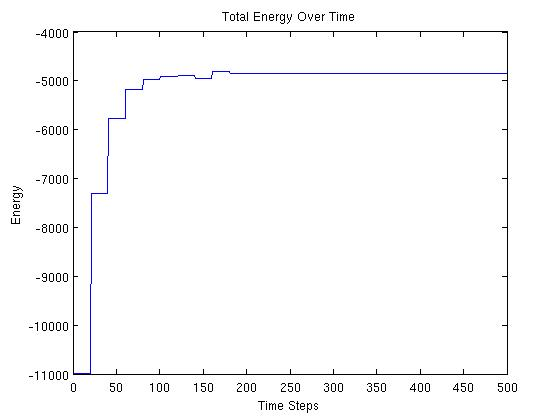
\includegraphics[width=0.8\linewidth]{energy2scale}
	\caption[Energy with temperature set to 2]{}
	\label{fig:energy2scale}
\end{figure}

Figure~\ref{fig:kenergy2scale} shows the Kinetic energy of the system over several time steps


\begin{figure}
	\centering
	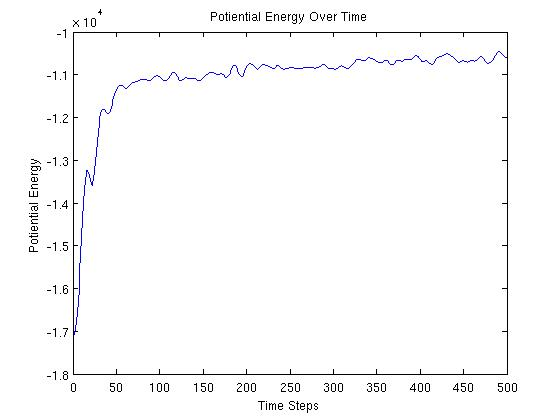
\includegraphics[width=0.8\linewidth]{penergy2scale}
	\caption[Energy with temperature set to 2]{}
	\label{fig:penergy2scale}
\end{figure}

Figure ~\ref{fig:penergy2scale} shows the potential energy of the system over several time steps 

\begin{figure}
	\centering
	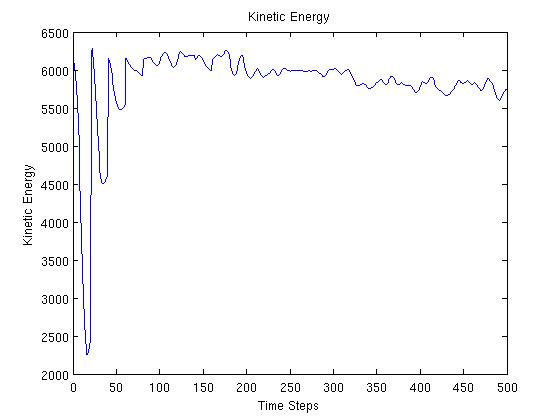
\includegraphics[width=0.8\linewidth]{kenergy2scale}
	\caption[Energy with temperature set to 2]{}
	\label{fig:kenergy2scale}
\end{figure}

\section{Temperature}
The temperature of the system is calculated using the Kinetic Energy:

$$ \sum_{i=1}^N \frac{|P_i|^2}{2 m_i} = \frac{k_B T}{2} (3N -3)$$

The following code is used to calculate the temperature

\begin{lstlisting}
	 ke = .5d0*sum(vel_prtl**2)
	 T = ke/(1.5d0*dble(numprtl-1))
\end{lstlisting}


Figure \ref{fig:temp1scale} shows the temperature when set to 1.0 with temperature scaling every 20 time steps until the 250th time step. 
\begin{figure}
\centering
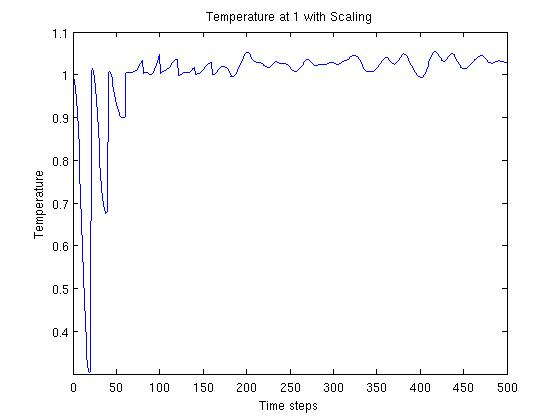
\includegraphics[width=0.8\linewidth]{temp1scale}
\caption[Temperature set to 1 with Temperature Scaling]{}
\label{fig:temp1scale}
\end{figure}
Figure \ref{fig:temp2scale} shows the temperature when set to 2.0 with scaling every 20 time steps until 250th time steps
\begin{figure}
	\centering
	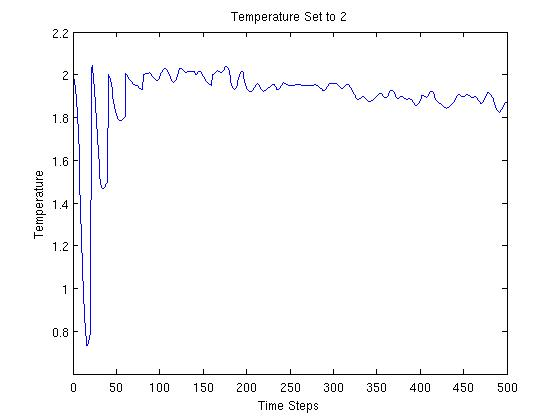
\includegraphics[width=0.8\linewidth]{temp2scale}
	\caption[Temperature set to 2 with Temperature Scaling]{}
	\label{fig:temp2scale}
\end{figure}

\section{Pressure}
The pressure of the system is calculated using the following:

$$ P=\frac{1}{V}[NK_BT - \frac{1}{3K_BT}\sum_{i=1}^{N-1}\sum_{j=1+1}^{N}r_{ij}f_{ij} ]  $$

The code for this routine is the following:

\begin{lstlisting}
press_temp = press_temp + sqrt(drsq)*sqrt(dot_product(force_mag*dr,force_mag*dr))
vol = boundry**(3.d0)
pressure = (numprtl*temp_m - (1.d0/(3.d0*temp_m))*pressure_temp)/vol
\end{lstlisting}

The product of the radius and the force is calculated in the force routine. The actually pressure value is calculated outside the force routine after the velocities are calculated. This is due to the temperatures dependency on the velocities. 

Figure \ref{fig:oressyre2scale} shows the pressure over time with temperature scaling of 2 degrees.  

\begin{figure}
	\centering
	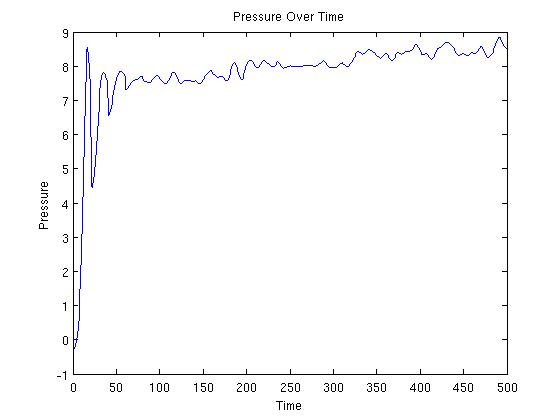
\includegraphics[width=0.8\linewidth]{pressure2scale}
	\caption[Pressure of the system ]{}
	\label{fig:oressyre2scale}
\end{figure}

\section{Radial Distribution Function}

The radial distribution function, plots the distribution of particles distances from each other. These distributions are averaged over time once the simulation becomes stable. Figure \ref{fig:raddistfunc2} shows the distribution averaged over the last 250 time steps of a 500 time step simulation. The temperature was set to 2 

\begin{figure}
	\centering
	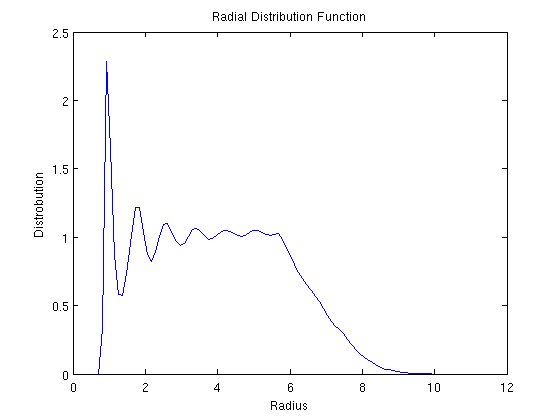
\includegraphics[width=0.8\linewidth]{raddistfunc2}
	\caption[Pressure of the system ]{}
	\label{fig:raddistfunc2}
\end{figure}
 

\end{document}